\section{基于锁的协议}

\subsection{基于锁的协议}

可串行化调度是并发控制的基础。

数据锁可以两种模式加锁:
\begin{enumerate}
    \item 排他(X)模式:数据项可以被读取和写入。使用lock-X指令请求X锁。
    \item 共享(S)模式:数据项只能被读取。使用lock-S指令请求S锁。
\end{enumerate}

锁请求发送给并发管理器。只有在请求被批准后,事务才能继续进行。

如果请求的锁与其它事务已持有的该项目上的锁兼容,则事务可能会被授予该项目的锁。

任意数量的事务可以在一个项目上持有共享锁。但是,如果任何事务持有该项目的排他锁,则其他事务不能在该项目上持有任何锁。

如果无法授予锁,则请求事务将被要求等待,直到其它事务持有的所有不兼容锁都被释放。然后再授予该锁。

加锁协议是所有事务在请求和释放锁时遵循的一组规则。加锁协议限制了可能的调度集合。

\subsection{基于锁的协议的陷阱}

考虑如下部分调度:

\begin{figure}[H]
    \centering
    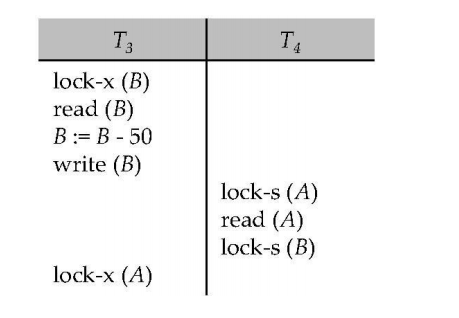
\includegraphics[width=0.7\linewidth]{image1.png}
    \caption{}
    \label{}
\end{figure}

$T_3$和$T_4$都无法取得进展——执行锁$S(B)$会使$T_4$等待$T_3$释放其对$B$的锁,
而执行锁$-X(A)$会使$T_3$等待$T_4$释放其对$A$的锁。这种情况称为死锁。

要处理死锁,必须回滚$T_3$或$T_4$中的一个并释放其锁。

大多数锁定协议都存在死锁的可能性,死锁是不可避免的问题。

如果并发控制管理器设计不当,也可能出现饥饿现象。例如:一个事务可能正在等待某个项目加排他锁,
而其它一系列事务却在请求并授予对同一项目的共享锁。同一事务由于死锁而反复回滚。

可以设计并发控制管理器来防止饥饿现象。

\subsection{两阶段锁协议}

这是一种确保冲突可串行化调度的协议。

阶段1:增长阶段。事务可以获取锁,事务不能释放锁。

阶段2:收缩阶段。事务可能会释放锁,事务可能无法获取锁。

该协议确保可串行性。可以证明,事务可以按照其锁点(即事务获取其最后一个锁的点)的顺序进行串行化。

两阶段锁不能确保避免死锁。

在两阶段锁机制下,级联回滚是可能发生的。为避免这种情况,可采用一种改进的协议,即严格两阶段锁协议。在该
协议中,事务必须持有其所有排他锁,直到提交或中止。

严格两阶段锁协议更为严格:在此协议中,所有锁都要持有到事务提交或中止。在这个协议中,事务可以按照提交
的顺序进行系列化。

如果使用两阶段锁,可能会存在无法得到的冲突可串行化调度。

然而,在没有额外信息(例如,对数据的访问顺序)的情况下,两阶段锁在以下意义上是实现冲突可串行化所必须的:
给定一个不遵循两阶段的事务$T_i$,我们可以找到一个使用两阶段锁的事务$T_i$,以及一个针对$T_i$
和$T_j$的非冲突可串行化调度。

\subsection{锁转换}

带有锁转换的两阶段锁:
\begin{itemize}
    \item 第一阶段
       \begin{itemize}
          \item 可以对项获取共享锁
          \item 可以对项获取排他锁
          \item 可以将S锁转化为X锁(升级)
       \end{itemize}
    \item 第二阶段
       \begin{itemize}
          \item 可以释放S锁
          \item 可以释放X锁
          \item 可以将X锁转化为S锁(降级)
       \end{itemize}
\end{itemize}

该协议确保可串行性,但仍依赖程序员插入各种加锁指令。

\subsection{锁的自动获取}

事务$T_i$发出标准的读/写指令,无需显式的加锁调用

\noindent 操作read(D)按如下方式处理:
\begin{lstlisting}[style=sqlstyle]
if Ti has a lock on D then
    read(D)
else begin
    if necessary wait until no other
    transaction has a lock-X on D then
        grant Ti a lock-S on D;
        read(D)
    end    
\end{lstlisting}

\noindent write(D)按以下方式处理:
\begin{lstlisting}[style=sqlstyle]
if Ti has a lock-X on D then
    write(D)
else begin
    if necessary wait until no other trans.has any lock on D,
        if Ti has a lock-S on D then
            upgrade lock on D to lock-X
        else 
            grant Ti a lock-X on D
            write(D)
    end;    
\end{lstlisting}

所有锁在提交或中止后释放。

\subsection{锁的实现}

锁管理器可以实现为一个单独的进程,事务向该进程发送加锁和解锁请求。

锁管理器通过发送锁授予消息(或者在发生死锁的情况下,发送一条要求事务回滚的消息)来响应加锁请求。

请求事务会一直等待,直到其请求得到响应。

锁管理器维护一个称为锁表的数据结构,用于记录已授予的锁和待处理的请求。

锁表通常实现为一个内存的哈希表,以被锁定的数据项的名称作为索引。

\subsection{锁表}

黑色矩形表示已授予的锁,白色矩形表示等待中的请求。

锁表还会记录已授予或请求的锁的类型。

新请求被添加到数据项请求队列的末尾,若与所有先前的锁兼容,则被批准。

解锁请求会导致该请求被删除,并检查后续请求是否现在可以被批准。

如果事务中止,则该事务的所有等待或已批准的请求都将被删除:
锁管理器可以维护每个事务持有的锁列表,以高效实现此功能。

\subsection{基于图的协议}

基于图的协议是两阶段锁的一种替代方案。

对所有数据项的集合$D=\{d_1,d_2,...,d_h\}$施加偏序$\to$。如果$d_i\to d_j$,则任何同时访问
$d_i$和$d_j$的事务必须在访问$d_j$之前访问$d_i$。意味着集合$D$现在可以被视为一个有向无环图,称为数据库图。

树协议是一种简单的图协议。

\begin{enumerate}
    \item 只允许使用X锁
    \item $T_i$的第一个锁可以加在任何数据项上。随后,$T_i$只能在$Q$的父节点当前已被$T_i$锁定的情况下,才能锁定数据$Q$。
    \item 数据项可以在任何时候解锁
    \item 一个已被$T_i$锁定并解锁的数据项,随后不能再由$T_i$重新锁定。
\end{enumerate}

优点:树形协议可确保冲突可串行化,且不会产生死锁。与两阶段锁协议相比,树形锁定协议中的解锁操作可能会
更早发生:等待时间更短,并发度提高;协议无死锁,无需回滚。

缺点:协议不保证可恢复性或无级联性——需要引入提交依赖关系以确保可恢复性——事务可能需要锁定它们不访问的数据项。
——增加了锁定开销和额外的等待时间——并发度可能降低。在两阶段锁定下不可能的调度在树协议下是可能的,反之亦然。